\documentclass[undgrad,numbers]{Controle/DES}
\usepackage[utf8]{inputenc}
\usepackage{amsmath,amssymb}
\usepackage{epigraph}
\usepackage{hyperref}
\usepackage{indentfirst}
%\usepackage{csquotes}
\usepackage{tikz}
\usepackage{longtable}
\usepackage[refpage]{nomencl}
\usepackage{lettrine}
\usepackage{multirow}
\usepackage{array}
\usepackage{tikz}
\usepackage[RPvoltages, american, cuteinductors,smartlabels]{circuitikz}
%\usepackage[]{circuitikz}
\usepackage{color, colortbl}
\usepackage{ctable}
%\setlength{\arrayrulewidth}{0.5mm}
\usepackage[document]{ragged2e}
\usepackage{lmodern}
\usepackage{pdfpages}
\usepackage[font=footnotesize,labelfont=bf]{caption}
\usepackage{fancyhdr}
\usepackage{ifthen}

\pagestyle{fancyplain}
\fancyhf{}
\fancyhead[R]{\thepage}
\renewcommand{\headrulewidth}{0pt}

\makelosymbols
\makeloabbreviations
\justifying

\begin{document}
\title{Primeiro projeto de Eletronica Digital} %Máximo de 4 linhas
\foreigntitle{My great title in english here}
\author{Bruno Franca - bruno.francaguimaraes@ufpe.br
  \\ Gabriela Leite - gabriela.lpereira@ufpe.br
  \\ Henrique da Silva - henrique.pedro@ufpe.br
  \\ Pedro Souza - pedro.souzaleao@ufpe.br}{} %Nome do(a) autor(a)

\advisor{Prof.}{Nomea do(a) Orientador(a)}{D.Sc.} %Nome do(a) orientador(a)
\newcommand{\exinsto}{Universidade Federal de Pernambuco} %IES do Orientador

\coadvisor{Prof.}{Nome do(a) Coorientador(a)}{D.Sc.}
% Coloque % no segundo examinador, caso não tenha.
% Coloque % no Coorientador, caso não tenha.

\examiner{Prof.}{Nome do(a) primeiro(a) examinador(a)}{D.Sc.}
\newcommand{\exinstum}{Universidade Federal de Pernambuco} %IES do primeiro examinador

\examiner{Prof.}{Nome do(a) segundo(a) examinador(a)}{Ph.D.}
\newcommand{\exinstdois}{Universidade Federal de Pernambuco} %IES do segundo examinador

\department{DES-ELE} % DES-TEL para Telecomunicações
\date{\the\month}{\the\year}

\newcommand{\Datadadefesa}{xx/xx/20xx}%Coloque a data da defesa dd/mm/aaaa

\mainmatter
% {Arquivos/dedic} %Dedicatória
% \thispagestyle{empty}
\Huge
\textbf{Agradecimentos}
\normalsize
\vspace{1cm}

%Início dos agradecimentos
Muitos agradecimentos a várias pessoas aqui.

\textcolor{red}{[Agradecimentos é um elemento opcional]} %Agradecimentos
\thispagestyle{empty}
\mbox{}\vfill
\epigraph{What I cannot create, I do not understand}{Richard Feynman}
% \textcolor{red}{[Epígrafe é um elemento opcional]}
 %Epígrafe
\begin{abstract}

O resumo do trabalho tem a finalidade de dar uma visão rápida ao leitor, para que ele possa decidir sobre a conveniência da leitura do texto inteiro. Ele tem que ser totalmente fiel ao trabalho e não pode conter nenhuma informação que não conste do texto integral. A primeira frase do resumo deve ser significativa, explicando o tema principal do documento. Não devem constar do resumo citação de autores, tabelas e figuras. O resumo precisa estar contido em um único parágrafo e em uma única página. De acordo com a norma da ABNT NBR 6028, o resumo deve conter até 500 palavras. Ao final, devem ser incluídas, por recomendação, entre três e cinco palavras-chave.

\palavraschave{Suspendisse; orci; iaculis; dignissim.}\\
\textcolor{red}{Obs: Palavras-chave separadas por ponto e vírgula, ponto no final e em minúsculas (com exceção dos substantivos próprios e nomes científicos).}

\end{abstract}
 %Resumo em português
\begin{foreignabstract}

Class aptent taciti sociosqu ad litora torquent per conubia nostra, per inceptos himenaeos. Nullam tempus interdum arcu, sed ullamcorper ipsum tempor et. Integer fermentum aliquam arcu, vel condimentum purus tincidunt id. Ut purus est, lobortis eu nisi sed, efficitur aliquam neque. Vestibulum vestibulum malesuada ante, vitae molestie erat ullamcorper vel. Mauris semper vestibulum est id bibendum. Quisque vehicula at purus id dapibus. Sed ornare, est ut luctus ultricies, odio justo pretium ipsum, et maximus lectus orci in libero. Sed sit amet lacus at odio ullamcorper convallis sit amet sed lacus.

\keywords{Digital Communications; Acoustic Communications; FPGA; Hardware Coprocessor.}\\
\textcolor{red}{Obs: Palavras-chave em inglês separadas por ponto e vírgula, ponto no final e em minúsculas (com exceção dos substantivos próprios e nomes científicos).}

\end{foreignabstract}
 %Resumo em inglês 

\addtocontents{toc}{\protect\thispagestyle{empty}}
\tableofcontents
\thispagestyle{empty}

\listoffigures %Gerar a lista de Ilustrações
\listoftables %Gerar a lista de Tabelas
\thispagestyle{empty}
\Huge
\textbf{Lista de Símbolos}
\normalsize
\vspace{1cm}

\begin{longtable}{lr}
A&\dotfill     Ampère\\
e&\dotfill      Constante de Euler ou Constante de Napier\\
E&\dotfill      Energia
\end{longtable}
  %Gerar a lista de Símbolos
\thispagestyle{empty}
\Huge
\textbf{{Lista de Abreviações}}
\normalsize
\vspace{1cm}

\begin{longtable}{lr}
    AD&\dotfill Analógico-para-Digital\\
    bps	&\dotfill bits por segundo  \\
    CI	&\dotfill Circuito Integrado  \\
    DA	&\dotfill Digital-para-Analógico
\end{longtable}
  %Gerar a lista de Abreviaturas

\pagestyle{plain}
\chapter{Introdução}
\label{cap:um}

\lettrine[loversize=0.25,findent=0.2em,nindent=0em]{I}{ntrodução}  é a apresentação rápida do assunto abordado e seu mérito. É uma seção na qual se aguça a curiosidade do leitor, na qual se tenta vender-lhe o projeto. É adequado terminar com a formulação do problema, sob a forma de pergunta.

Problematização é a transformação de uma necessidade humana em problema. Segundo Popper (1975), toda discussão científica deve surgir com base em um problema ao qual se deve oferecer uma solução provisória a que se deve criticar, de modo a eliminar o erro. É uma questão não resolvida, é algo para o qual se vai buscar resposta, via pesquisa. %\cite{lakatos2001trabalho}
(\citeauthor{lakatos2001trabalho}, \citeyear{lakatos2001trabalho})

Na introdução poderá ser incluída a metodologia usada na sua pesquisa, assim como um roteiro que deixe claro como está organizado o seu trabalho, como por exemplo: no capítulo 2 será abordado..., no capítulo 3 veremos como..., e assim por diante. É provável que só após a conclusão dos capítulos é que possamos acrescentar o roteiro...

Este modelo segue as orientações do modelo disponibilizado no site da UFPE (\citeauthor{Modelo_TCC}, \citeyear{Modelo_TCC}) . 


\section{Justificativa}\label{Motivação}
Justificar é oferecer razão suficiente para a construção do trabalho. Responde a pergunta por que fazer o trabalho, procurando os antecedentes do problema e a relevância do assunto/tema, argumentando sobre a importância prático teórica, colocando as possíveis contribuições esperadas.

(Aqui deve ser colocado o por quê do seu trabalho. Por que o seu trabalho é relevante? Por que você vai fazê-lo?)


\section{Objetivo Geral}\label{Objetivos}

Refere-se a indicação do que é pretendido com a realização do estudo ou pesquisa e quais os resultados que se pretende alcançar. Define o que se quer fazer na pesquisa. Os objetivos devem ser redigidos com verbos no infinitivo, exemplo: caracterizar, identificar, compreender, analisar, verificar.

Procura dar uma visão global e abrangente do tema, definindo de modo amplo, o que se pretende alcançar. Quando alcançado dá a resposta ao problema.

(Aqui deve ser colocado o que você pretende com o seu trabalho onde você quer chegar. Seria o: para quê? do seu trabalho.) 

\subsection{Objetivos específicos}\label{Objetivos específicos}
\begin{enumerate}
\item[$\bullet$] Analisar os diversos xyxyxyx  xyxyx xyxyyxyxyxyxyyxyyx;
\item[$\bullet$] Identificar as diversas hjdhfjh dhjfh djhfjhdjhfjjhdjhhjhfjhjdhf;
\item[$\bullet$] Verificar a possibilidade do ddjgklsjd gkjfgkjkjxg kldjkfg dkfjkgljdkflg;
\item[$\bullet$] kasjhdkjashdkjasdh askdhksajdh kjasdhk ashd kashd kjsahdk jashdkjh askjdh aksjdh kadshd;
\end{enumerate}

Os objetivos específicos tem função intermediária e instrumental, ou seja, tratam dos aspectos concretos que serão abordados na pesquisa e que irão contribuir para se atingir o objetivo geral. É com base nos objetivos específicos que o pesquisador irá orientar o levantamento de dados e informações.


\section{Organização do TCC}\label{Organização do TCC}

O conteúdo deste TCC está dividido em sete capítulos e um apêndice. As referências encontram-se nas páginas finais. A seguir, um resumo dos capítulos seguintes do TCC.

\begin{description}
    \item[Capítulo 2.] Donec a nisi lobortis, pretium nulla eu, ornare nulla. Nullam varius iaculis lacus, eu rutrum velit sollicitudin eu.     
    
    \item[Capítulo 3.] Donec a nisi lobortis, pretium nulla eu, ornare nulla. Nullam varius iaculis lacus, eu rutrum velit sollicitudin eu. 
    
    \item[Capítulo 4.] Donec a nisi lobortis, pretium nulla eu, ornare nulla. Nullam varius iaculis lacus, eu rutrum velit sollicitudin eu. 
    
    \item[Capítulo 5.] Donec a nisi lobortis, pretium nulla eu, ornare nulla. Nullam varius iaculis lacus, eu rutrum velit sollicitudin eu. 
    
    \item[Capítulo 6.] Donec a nisi lobortis, pretium nulla eu, ornare nulla. Nullam varius iaculis lacus, eu rutrum velit sollicitudin eu. 
    
    \item[Capítulo 7.] Donec a nisi lobortis, pretium nulla eu, ornare nulla. Nullam varius iaculis lacus, eu rutrum velit sollicitudin eu. 
    
    \item[Apêndice A.] Donec a nisi lobortis, pretium nulla eu, ornare nulla. Nullam varius iaculis lacus, eu rutrum velit sollicitudin eu. 

\end{description} %Gerar o Capítulo 1
\chapter{Fundamentação Teórica}
\label{cap:dois}


{\lettrine[loversize=0.25,findent=0.2em,nindent=0em]{A}{liquam} a malesuada magna, et placerat ex. Cras luctus, lorem sit amet semper ornare, nisi libero condimentum elit, ut finibus nunc est et nunc. Proin sollicitudin vulputate placerat. Nam et lacinia arcu, ac cursus neque. Integer facilisis dui nec nibh fringilla sagittis. Morbi blandit enim libero, in consectetur leo consequat ut. Suspendisse a orci id nibh egestas aliquet vel at leo. Etiam at venenatis leo, eget dignissim mi. Donec non justo in erat aliquam molestie eget quis erat. Sed aliquam velit non velit pharetra viverra. Suspendisse dapibus rhoncus ex, at varius ligula condimentum et. Orci varius natoque penatibus et magnis dis parturient montes, nascetur ridiculus mus. Morbi maximus lobortis auctor. Ut et metus lobortis, ultricies dolor et, posuere justo. Mauris a convallis quam. Mauris iaculis gravida ligula, sed viverra quam volutpat nec.

\section{Seção 1}\label{Seção 12}
Donec a nisi lobortis, pretium nulla eu, ornare nulla. Nullam varius iaculis lacus, eu rutrum velit sollicitudin eu. Mauris ultricies lacus vel lectus porta, non laoreet metus maximus. Cras porttitor tincidunt nunc, vel egestas sem. Etiam sit amet ultrices arcu. Sed et lacus quis ex vestibulum fringilla eget a odio. Morbi ut quam pharetra, mattis ipsum a, faucibus neque. Pellentesque laoreet risus eros, eu venenatis ipsum auctor sed. Donec vehicula porttitor nibh, ut sodales est imperdiet pretium. Phasellus quis accumsan odio, id consequat eros. Donec mauris neque, tincidunt vitae sapien finibus, hendrerit tincidunt eros. Integer volutpat sit amet sapien eu mollis. Aliquam erat volutpat. Maecenas porta porttitor mauris et tincidunt. (\citeauthor{smith2014microelectronic}, \citeyear{smith2014microelectronic})

\begin{figure}[h!]
  \caption{Conversor BOOST}
\begin{center}
\resizebox{0.8\textwidth}{!}{
\begin{circuitikz}
 \draw (6.4,-1.2) node[] {$+$};
 \draw (6.4,-1.5) node[] {$v_{o}$};
 \draw (6.4,-1.8) node[] {$-$};
 \draw (0,-3) -- (6,-3);
 \draw (0,-3) [V, l_=$v_{s}$] to (0,0); 
 \ctikzset{diodes/scale=0.6,resistors/scale=0.6}
 \draw (0,0) [L, l^=+ $v_L$ -, -*] to (2,0); 
 \draw (2,-1.8) to[short, *-*] (2,-3);
 \draw (2,0) to[short, -o] (2,-1.3);
 \draw (4,0) -- (6,0);
 \draw (2,0) [D, l^=$D$, *-*] to (4,0); 
 \draw (2,-3) [spst] to (2,0); 
 \draw (4,-3) [C, l_=$C$,*-*] to (4,0); 
 \draw (6,0) [R, l_=$R_L$] to (6,-3); 
 \draw (0.1,-0.1) to[open, f_>=$i_L$] (1.1,-0.1); 
 \draw (2.1,-0.1) to[open, f_>=$i_D$] (3.1,-0.1); 
 \draw (4,0) to[open, f^>=$i_C$] (4,-0.5); 
 \draw (6,0) to[open, f^>=$i_R$] (6,-0.5); 
\end{circuitikz}}\\
  {\footnotesize Fonte: O Autor(2023), adaptado de (\citeauthor{hart2016eletronica}, \citeyear{hart2016eletronica}).}  %Fonte um pouco menor que a do texto
  \label{6.8a.eps}
\end{center}
\end{figure}

Class aptent taciti sociosqu ad litora torquent per conubia nostra, per inceptos himenaeos. Nam porta est sed velit dignissim, ut fringilla est fringilla. Maecenas semper ut dui ac dignissim. Phasellus eu nisl sed diam pellentesque feugiat faucibus nec nisl. Vivamus in tempus dolor. Ut urna diam, lacinia in tincidunt sed, elementum quis velit. Morbi sapien elit, condimentum sed mi eu, ullamcorper tincidunt justo. Aliquam sollicitudin sollicitudin magna ac faucibus.


\section{Seção 2}\label{Seção 22}
Donec a nisi lobortis, pretium nulla eu, ornare nulla. Nullam varius iaculis lacus, eu rutrum velit sollicitudin eu. Mauris ultricies lacus vel lectus porta, non laoreet metus maximus. Cras porttitor tincidunt nunc, vel egestas sem. Etiam sit amet ultrices arcu. Sed et lacus quis ex vestibulum fringilla eget a odio. Morbi ut quam pharetra, mattis ipsum a, faucibus neque. Pellentesque laoreet risus eros, eu venenatis ipsum auctor sed. Donec vehicula porttitor nibh, ut sodales est imperdiet pretium. Phasellus quis accumsan odio, id consequat eros. Donec mauris neque, tincidunt vitae sapien finibus, hendrerit tincidunt eros. Integer volutpat sit amet sapien eu mollis. Aliquam erat volutpat. Maecenas porta porttitor mauris et tincidunt.

Class aptent taciti sociosqu ad litora torquent per conubia nostra, per inceptos himenaeos. Nam porta est sed velit dignissim, ut fringilla est fringilla. Maecenas semper ut dui ac dignissim. Phasellus eu nisl sed diam pellentesque feugiat faucibus nec nisl. Vivamus in tempus dolor. Ut urna diam, lacinia in tincidunt sed, elementum quis velit. Morbi sapien elit, condimentum sed mi eu, ullamcorper tincidunt justo. Aliquam sollicitudin sollicitudin magna ac faucibus.


\section{Seção 3}\label{Seção 32}
Donec a nisi lobortis, pretium nulla eu, ornare nulla. Nullam varius iaculis lacus, eu rutrum velit sollicitudin eu. Mauris ultricies lacus vel lectus porta, non laoreet metus maximus. Cras porttitor tincidunt nunc, vel egestas sem. Etiam sit amet ultrices arcu. Sed et lacus quis ex vestibulum fringilla eget a odio. Morbi ut quam pharetra, mattis ipsum a, faucibus neque. Pellentesque laoreet risus eros, eu venenatis ipsum auctor sed. Donec vehicula porttitor nibh, ut sodales est imperdiet pretium. Phasellus quis accumsan odio, id consequat eros. Donec mauris neque, tincidunt vitae sapien finibus, hendrerit tincidunt eros. Integer volutpat sit amet sapien eu mollis. Aliquam erat volutpat. Maecenas porta porttitor mauris et tincidunt.

\begin{table}
\caption{Coeficientes de $g_4(\alpha)$ para $g_4(\alpha)=\alpha^4+\alpha+1$, em $GF(16)$}
\newcolumntype{?}{!{\vrule width 2pt}}
\centering
\resizebox{0.7\textwidth}{!}{
\begin{tabular}{|c?c|c|c|c|c|c|c|c|c|c|c|c|c|c|c|}
\hline
$n-k$ & $g_{14}$ & $g_{13}$ & $g_{12}$ & $g_{11}$ & $g_{10}$ & $g_9$ & $g_8$ & $g_7$ & $g_6$ & $g_5$ & $g_4$ & $g_3$ & $g_2$ & $g_1$ & $g_0$ \\ \specialrule{2pt}{0pt}{0pt}
  $2$ &     &     &     &     &     &     &     &     &     &     &     &     &  $1$& $6$ & $8$ \\ \hline
  $3$ &     &     &     &     &     &     &     &     &     &     &     &  $1$& $14$& $13$& $12$ \\ \hline
  $4$ &     &     &     &     &     &     &     &     &     &     &  $1$& $13$& $12$& $8$ & $7$ \\ \hline 
  $5$ &     &     &     &     &     &     &     &     &     & $1$ & $11$& $4$ & $6$ & $2$ & $1$  \\ \hline
  $6$ &     &     &     &     &     &     &     &     & $1$ & $7$ & $9$ & $3$ & $12$& $10$& $12$ \\ \hline
  $7$ &     &     &     &     &     &     &     & $1$ & $12$& $13$& $15$& $2$ & $7$ & $14$& $13$ \\ \hline
  $8$ &     &     &     &     &     &     & $1$ & $9$ & $4$ & $3$ & $4$ & $13$& $6$ & $14$& $12$ \\ \hline
  $9$ &     &     &     &     &     & $1$ & $3$ & $1$ & $13$& $9$ & $3$ & $13$& $7$ & $10$& $1$  \\ \hline
 $10$ &     &     &     &     & $1$ & $4$ & $8$ &$10$ & $12$& $9$ & $4$ & $2$ & $12$& $2$ & $7$  \\ \hline
 $11$ &     &     &     & $1$ & $10$ & $5$ & $3$ &$10$ & $13$& $3$ & $15$& $3$ & $6$ & $8$ & $12$ \\ \hline
 $12$ &     &     & $1$ & $5$ & $9$ & $5$ & $8$ & $1$ & $4$ & $13$& $9$ & $4$ & $12$& $13$& $8$  \\ \hline
 $13$ &     & $1$ & $8$ & $5$ & $10$ & $4$ & $3$ & $9$ & $12$& $7$ & $11$& $13$& $14$& $6$ & $2$  \\ \hline
 $14$ & $1$ & $1$ & $1$ & $1$ & $1$ & $1$ & $1$ & $1$ & $1$ & $1$ & $1$ & $1$ & $1$ & $1$ & $1$  \\ \hline

\end{tabular}}\\
{\footnotesize Fonte: O Autor(2023).}
\label{tab:coeficientes de gk(x)}
\end{table}

Class aptent taciti sociosqu ad litora torquent per conubia nostra, per inceptos himenaeos. Nam porta est sed velit dignissim, ut fringilla est fringilla. Maecenas semper ut dui ac dignissim. Phasellus eu nisl sed diam pellentesque feugiat faucibus nec nisl. Vivamus in tempus dolor. Ut urna diam, lacinia in tincidunt sed, elementum quis velit. Morbi sapien elit, condimentum sed mi eu, ullamcorper tincidunt justo. Aliquam sollicitudin sollicitudin magna ac faucibus.


\subsection{Subseção 1}\label{Subseção 12}
Donec a nisi lobortis, pretium nulla eu, ornare nulla. Nullam varius iaculis lacus, eu rutrum velit sollicitudin eu. Mauris ultricies lacus vel lectus porta, non laoreet metus maximus. Cras porttitor tincidunt nunc, vel egestas sem. Etiam sit amet ultrices arcu. Sed et lacus quis ex vestibulum fringilla eget a odio. Morbi ut quam pharetra, mattis ipsum a, faucibus neque. Pellentesque laoreet risus eros, eu venenatis ipsum auctor sed. Donec vehicula porttitor nibh, ut sodales est imperdiet pretium. Phasellus quis accumsan odio, id consequat eros. Donec mauris neque, tincidunt vitae sapien finibus, hendrerit tincidunt eros. Integer volutpat sit amet sapien eu mollis. Aliquam erat volutpat. Maecenas porta porttitor mauris et tincidunt.

\begin{figure}[h!]
\caption{Formas de onda.}
\begin{center}
  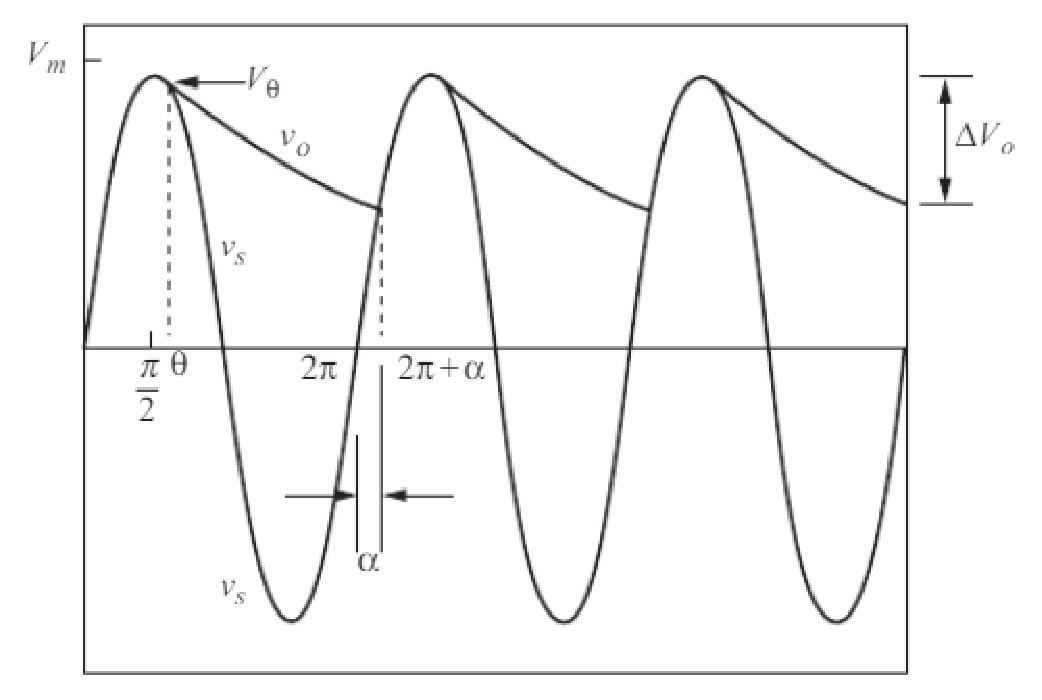
\includegraphics[width=7cm]{Ilustrações/Forma_de_onda.eps}\\
  {\footnotesize Fonte: (\citeauthor{hart2016eletronica}, \citeyear{hart2016eletronica}).}
  \label{3.2b.eps}
\end{center}
\end{figure}

Class aptent taciti sociosqu ad litora torquent per conubia nostra, per inceptos himenaeos. Nam porta est sed velit dignissim, ut fringilla est fringilla. Maecenas semper ut dui ac dignissim. Phasellus eu nisl sed diam pellentesque feugiat faucibus nec nisl. Vivamus in tempus dolor. Ut urna diam, lacinia in tincidunt sed, elementum quis velit. Morbi sapien elit, condimentum sed mi eu, ullamcorper tincidunt justo. Aliquam sollicitudin sollicitudin magna ac faucibus.




 %Gerar o Capítulo 2
\chapter{Desenvolvimento}
\label{cap:tres}

{\lettrine[loversize=0.25,findent=0.2em,nindent=0em]{N}{ulla} erat urna, tincidunt ut purus quis, cursus vulputate orci. Etiam est eros, vulputate vitae eros vitae, dapibus consequat augue. Fusce porta libero eu condimentum finibus. Vivamus euismod vestibulum arcu, ut eleifend quam sollicitudin vel. Orci varius natoque penatibus et magnis dis parturient montes, nascetur ridiculus mus. Nullam velit neque, pulvinar quis mauris vitae, lobortis malesuada neque. Aenean eget faucibus lacus.

In lobortis turpis vitae efficitur vestibulum. Sed ac scelerisque risus, at consectetur eros. Curabitur congue velit sit amet massa lacinia, ut aliquet velit vulputate. Suspendisse ut porta ligula. Suspendisse id porttitor leo. Duis rhoncus consectetur pretium. Fusce finibus justo neque, in blandit libero interdum eget. Fusce pretium condimentum dolor, et feugiat eros feugiat vitae.

\section{Sistema Proposto}

In blandit diam ac ipsum aliquam, ac sollicitudin magna maximus. Fusce placerat aliquam velit vitae condimentum. Morbi malesuada fringilla diam, nec vulputate ligula posuere in. Praesent lobortis suscipit ullamcorper. Praesent efficitur eros nec euismod mattis. Sed faucibus, massa eget egestas maximus, libero lacus egestas sapien, non varius purus elit faucibus nunc. Praesent a ex sit amet ex auctor elementum.

Sed a libero eget elit facilisis fermentum. Aliquam pharetra, ex a pharetra hendrerit, turpis ipsum egestas nisl, eget blandit tortor ipsum sit amet elit. Pellentesque hendrerit molestie lectus ac egestas. Pellentesque id diam est. Praesent libero risus, tristique a tortor id, malesuada placerat est. Quisque venenatis eros non dui volutpat, vel pulvinar diam fermentum. 
 %Gerar o Capítulo 3
\chapter{Considerações Finais}
\label{cap:conclusoes}

{\lettrine[loversize=0.25,findent=0.2em,nindent=0em]{N}{am} turpis odio, eleifend non finibus eu, ullamcorper vitae arcu. Praesent feugiat euismod massa, in tempor leo ultricies eget. Donec eget lacus vel nunc pretium placerat. Morbi elementum convallis enim, id ultricies metus pharetra ut. Maecenas enim ligula, viverra a dignissim vehicula, condimentum euismod mi. Vestibulum ante ipsum primis in faucibus orci luctus et ultrices posuere cubilia Curae; Sed sed turpis non purus elementum porta non vitae sem.

Nulla imperdiet augue ac diam tincidunt, ut varius sem luctus. Morbi vehicula imperdiet diam ac sollicitudin. In porta libero vitae tortor vestibulum, et dignissim arcu bibendum. Maecenas fermentum magna turpis, at dapibus libero bibendum ac.

\section{Conclusão}

Nulla egestas volutpat nisi vitae hendrerit. Suspendisse arcu orci, iaculis non mi sit amet, cursus dignissim enim. Sed convallis auctor odio, ac imperdiet tellus rutrum nec. Mauris tempus metus urna, et iaculis enim vestibulum nec. Morbi ullamcorper ipsum tellus, in feugiat urna pharetra eget.

Duis a felis lacinia, interdum nulla ut, tempus lacus. Nullam sodales eu tellus ut suscipit. Ut ut sollicitudin diam, vulputate sodales mi. Nulla venenatis diam nunc, non consequat enim maximus at. Cras congue tortor lorem, quis aliquet erat facilisis quis. Aliquam lobortis, quam eget malesuada bibendum, massa nulla imperdiet augue, vel porttitor elit tortor et felis.

\section{Dificuldades Encontradas}

Nulla egestas volutpat nisi vitae hendrerit. Suspendisse arcu orci, iaculis non mi sit amet, cursus dignissim enim. Sed convallis auctor odio, ac imperdiet tellus rutrum nec. Mauris tempus metus urna, et iaculis enim vestibulum nec. Morbi ullamcorper ipsum tellus, in feugiat urna pharetra eget.

Duis a felis lacinia, interdum nulla ut, tempus lacus. Nullam sodales eu tellus ut suscipit. Ut ut sollicitudin diam, vulputate sodales mi. Nulla venenatis diam nunc, non consequat enim maximus at. Cras congue tortor lorem, quis aliquet erat facilisis quis. Aliquam lobortis, quam eget malesuada bibendum, massa nulla imperdiet augue, vel porttitor elit tortor et felis.

\section{Trabalhos Futuros}

Nulla egestas volutpat nisi vitae hendrerit. Suspendisse arcu orci, iaculis non mi sit amet, cursus dignissim enim. Sed convallis auctor odio, ac imperdiet tellus rutrum nec. Mauris tempus metus urna, et iaculis enim vestibulum nec. Morbi ullamcorper ipsum tellus, in feugiat urna pharetra eget.

\begin{enumerate}
\item[$\bullet$] Implementar novos sensores... xyxyxyx  xyxyx xyxyyxyxyxyxyyxyyx;
\item[$\bullet$] Realizar... hjdhfjh dhjfh djhfjhdjhfjjhdjhhjhfjhjdhf;
\item[$\bullet$] Desenvolver uma versão... ddjgklsjd gkjfgkjkjxg kldjkfg dkfjkgljdkflg;
\item[$\bullet$] kasjhdkjashdkjasdh askdhksajdh kjasdhk ashd kashd kjsahdk jashdkjh askjdh aksjdh kadshd;
\end{enumerate}
 %Gerar o Capítulo 4 (Se precisar, crie o arquivo Arquivos/chap05 para o capítulo 5 e assim por diante e inclua uma linha para cada capítulo adicionado)
\backmatter
\bibliography{Arquivos/DES}

\appendix % Coloque % nesta linha caso não tenha Apêndices
\addcontentsline{toc}{chapter}{Apêndices}%

\chapter{Título do Apêndice A}

Morbi nunc tellus, molestie et urna quis, blandit dapibus felis. Morbi semper condimentum nulla, in mattis nulla lobortis eget. Cras pretium dapibus ullamcorper. Morbi porta quis dui non volutpat. Donec feugiat sem risus. Fusce cursus neque quis molestie accumsan. Quisque lobortis purus orci, sed placerat nulla sodales vitae. Proin condimentum, nibh in aliquet mollis, eros orci dictum libero, id congue erat neque nec nulla.

Quisque sem tortor, lacinia nec tincidunt eu, efficitur vel ex. In nec leo quis justo condimentum vulputate vel ut lorem. Integer eu metus quis mi dignissim sodales. Phasellus vestibulum ex vitae nisl interdum, ut fringilla arcu dapibus. Suspendisse tristique sed nisi quis ullamcorper. Proin eu tincidunt massa.
 % Coloque % nesta linha caso não tenha o Apêndice A
\chapter{Título do Apêndice B}

Morbi nunc tellus, molestie et urna quis, blandit dapibus felis. Morbi semper condimentum nulla, in mattis nulla lobortis eget. Cras pretium dapibus ullamcorper. Morbi porta quis dui non volutpat. Donec feugiat sem risus. Fusce cursus neque quis molestie accumsan. Quisque lobortis purus orci, sed placerat nulla sodales vitae. Proin condimentum, nibh in aliquet mollis, eros orci dictum libero, id congue erat neque nec nulla.

Quisque sem tortor, lacinia nec tincidunt eu, efficitur vel ex. In nec leo quis justo condimentum vulputate vel ut lorem. Integer eu metus quis mi dignissim sodales. Phasellus vestibulum ex vitae nisl interdum, ut fringilla arcu dapibus. Suspendisse tristique sed nisi quis ullamcorper. Proin eu tincidunt massa.
 % Coloque % nesta linha caso não tenha o Apêndice B
%(Se precisar, crie o arquivo Arquivos/ApendiceC para o apêndice C e assim por diante e inclua uma linha para cada apêndice adicionado)

\anexos  % Coloque % nesta linha caso não tenha anexos
\addcontentsline{toc}{chapter}{Anexos}%

\chapter{Título do Anexo A}

Morbi nunc tellus, molestie et urna quis, blandit dapibus felis. Morbi semper condimentum nulla, in mattis nulla lobortis eget. Cras pretium dapibus ullamcorper. Morbi porta quis dui non volutpat. Donec feugiat sem risus. Fusce cursus neque quis molestie accumsan. Quisque lobortis purus orci, sed placerat nulla sodales vitae. Proin condimentum, nibh in aliquet mollis, eros orci dictum libero, id congue erat neque nec nulla.

Quisque sem tortor, lacinia nec tincidunt eu, efficitur vel ex. In nec leo quis justo condimentum vulputate vel ut lorem. Integer eu metus quis mi dignissim sodales. Phasellus vestibulum ex vitae nisl interdum, ut fringilla arcu dapibus. Suspendisse tristique sed nisi quis ullamcorper. Proin eu tincidunt massa.
 % Coloque % nesta linha caso não tenha o Anexo A
\chapter{Título do Anexo B}

Morbi nunc tellus, molestie et urna quis, blandit dapibus felis. Morbi semper condimentum nulla, in mattis nulla lobortis eget. Cras pretium dapibus ullamcorper. Morbi porta quis dui non volutpat. Donec feugiat sem risus. Fusce cursus neque quis molestie accumsan. Quisque lobortis purus orci, sed placerat nulla sodales vitae. Proin condimentum, nibh in aliquet mollis, eros orci dictum libero, id congue erat neque nec nulla.

Quisque sem tortor, lacinia nec tincidunt eu, efficitur vel ex. In nec leo quis justo condimentum vulputate vel ut lorem. Integer eu metus quis mi dignissim sodales. Phasellus vestibulum ex vitae nisl interdum, ut fringilla arcu dapibus. Suspendisse tristique sed nisi quis ullamcorper. Proin eu tincidunt massa.
 % Coloque % nesta linha caso não tenha o Anexo B
%(Se precisar, crie o arquivo Arquivos/AnexoC para o anexo C e assim por diante e inclua uma linha para cada anexo adicionado)

\end{document}
